\documentclass[conference]{IEEEtran}
\IEEEoverridecommandlockouts
% The preceding line is only needed to identify funding in the first footnote. If that is unneeded, please comment it out.
\usepackage{cite}
\usepackage{amsmath,amssymb,amsfonts}
\usepackage{algorithmic}
\usepackage{graphicx}
\usepackage{textcomp}
\usepackage{xcolor}
\usepackage{float}

\def\BibTeX{{\rm B\kern-.05em{\sc i\kern-.025em b}\kern-.08em
    T\kern-.1667em\lower.7ex\hbox{E}\kern-.125emX}}
\begin{document}

\title{Medical Image Synthesis with \\Pix2Pix Generative Adversarial Networks}


\author{\IEEEauthorblockN{1\textsuperscript{st} Aditya Nath}
\IEEEauthorblockA{\textit{Computer Science} \\
\textit{Indiana University South Bend}\\
South Bend, IN, USA}
\and
\IEEEauthorblockN{2\textsuperscript{nd} Jay Patel}
\IEEEauthorblockA{\textit{Computer Science} \\
\textit{Indiana University South Bend}\\
South Bend, IN, USA}
\and
\IEEEauthorblockN{3\textsuperscript{rd} James Amo}
\IEEEauthorblockA{\textit{Computer Science} \\
\textit{Indiana University South Bend}\\
South Bend, IN, USA}
}

\maketitle

\begin{abstract}
    Abstract
One of the growing areas in Deep Learning is the medical image classification. However, medical images are scarce and difficult to come by due to legal concerns regarding patient privacy.  Generative Adversarial Networks (GAN) and its extensions have opened some interesting ways to tackle these well-knowing challenges in medical images.
Generative Adversarial Networks are based on an adversarial process where one network is generating artificial images, while the other network continuously learns to differentiate between real and fake images. Because GANs can synthesize images at unprecedented levels of realism, we can use it to solve some of the scarcity of labeled data in the medical field. 
In our project, we used Pix2Pix Generative Adversarial Network which is a type of conditional Generative Adversarial Network (CGAN), where the generation of the output image is conditional on an input. The discriminator is presented with both a source image and the target image and must determine whether the target is a credible transformation of the source image.
\end{abstract}

\begin{IEEEkeywords}
generative adversarial network, image synthesis, Pix2Pix GAN, perceptual loss function
\end{IEEEkeywords}

\section{Introduction}
In 2014 Ian Goodfellow et al., proposed adversarial nets framework in which the generative model is pitted against an adversary: a discriminative model that learns to determine whether a sample is from a model distribution or the data distribution \cite{goodfellow2014generative}. Later, in the year Mehdi Mirza et al, proposed a conditional version of the generative adversarial nets, which can be constructed by simply feeding the data, y, we wish to condition on to both the generator and discriminator \cite{mirza2014conditional}.

Pix2Pix model is a type of conditional GAN, whereby the generation of the image is conditional on an input, which in this case a source image. The discriminator is provided both the a source image and the target image and must determine whether the target is a plausible transformation of the source image \cite{pix2pix_ml}. Conditional GAN is very similar to GAN, except both the generator and discriminator are conditioned on some extra information. Figure \ref{fig:gan} shows the GAN architecture whilst Figure \ref{fig:condtionalgan} shows the Conditional GAN architecture. The Pix2Pix GAN has been demonstrated on a range of image-to-image translation tasks such as converting maps to satellite photographs, black and white photographs to color, and sketches of products to product photographs \cite{conditional_gan_explain}.

\begin{figure}[htbp]
    \centering
    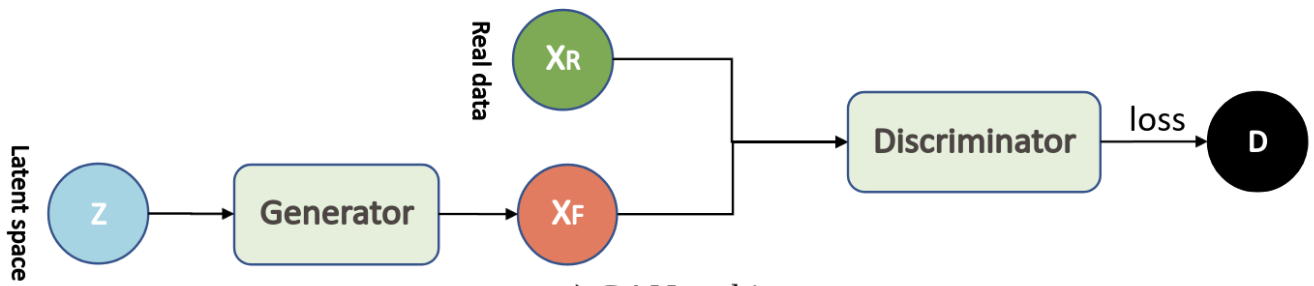
\includegraphics[width=\columnwidth]{gan.png}
    \caption{GAN Architecture \protect\cite{conditional_gan_explain}}
    \label{fig:gan}
\end{figure}

\begin{figure}[htbp]
    \centering
    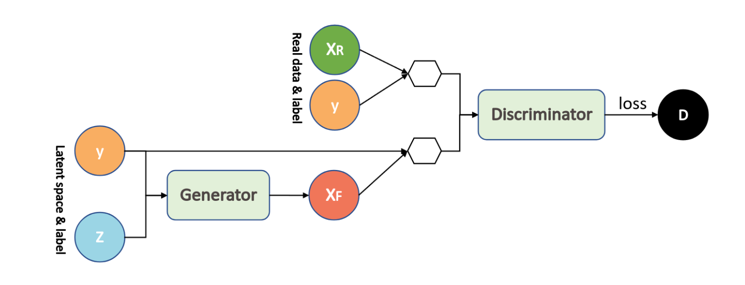
\includegraphics[width=\columnwidth]{cgan.png}
    \caption{Conditional GAN Architecture \protect\cite{conditional_gan_explain}}
    \label{fig:condtionalgan}
\end{figure}

By adding the label data, y, to both the generator and the discriminator forces the network to operate in a certain mode. For example, instead of just asking the generator to generate digits from 0-9 using the MNIST sample, the generator can be told to only output a certain number, let say 5 and ask the discriminator whether the particular output image is 5.

\section{Build and Training}

\subsection{Training Datasets}

The MNIST handwritten digits dataset was initially used to test the algorithm. We then use the T1 \& T2 medical images from IXI Datasets \cite{dataset_ixi} made available under the Creative Commons CC BY-SA 3.0 license. The images were downloaded and processed using the nibabel package (https://nipy.org/nibabel/). We wrote a script which extract data from the .nii.gz files. From T1, we only gather instances with 150 slices. From T2, we only gather instances with 130 slices. We did this because those are the number of slices that occurs maximum number of times in the entire dataset. For each, we selected the middle 90-110 slices for our experiment.

\subsection{Training}
Training for this model relies on a discriminator identifying predicted truth images as fake and then generator using this perceived “loss” to generate images as close to the target domain as possible. This particular overall inferred loss mechanism is known as an adversarial loss function. 

Using the model described in \cite{pix2pix_ml}, we worked with a paired dataset, were we are sure of a direct correlation between the images. We also assumed that the direct correlation between the images will hold true for adjacent slices, thus we decided to include 20 neighboring slices in the training instead of a single slice. For the generator, the training would involve feeding it only noise and then allowing it to learn from the feedback from the discriminator. However in this generator, we introduced randomness in another way, that is, by adding a dropout layer. The mechanism used by the generator, also known as UNet generator, where the input is downsampled for a certain number of layers by using a deep convolutional layer of stride 2 and is then upsampled for the equal number of layers, using a transpositional convolutional network with the modification of using skip connections. For training the discriminator, we use a patchGAN model\cite{pix2pix_ml} which uses a $70 \times 70$ patch on the generated or real images, in a convolutional manner, to determine the classification of the image.

In the training process, the  Generator $G$ takes $x$ and $z$ then it produces $y$. The goal of the G is to produce output images that cannot be distinguished from “real” images by the discriminator. The discriminator $D$, on the other hand, takes the pair ($x$ and $y$) from both real images and fake images and distinguish between them as either fake or real inputs.

Training Pix2Pix GAN as the same as training any other GAN except a little modification that is being done at the generator’s loss function. The generator $G$ is not only trying to reduce the loss from discriminator but also trying to move the fake distribution close to real distribution by using $L1$ or $L2$ loss. See \cite{isola2016imagetoimage} for details of $L1$ and $L2$ mathematical equations. The perceptual loss function was used for this model which works by summing all the squared errors between all the pixels and taking the mean. This is in contrast to a per-pixel loss function which sums all the absolute errors between pixels.

\section{Results and Observations} % \label{AA}
To get accustomed to the model and understand it well, we trained the model using the MNIST datasets. After training it for 20000 epochs, the output of the generated images was closed to the real image. With some modifications to the model, we adopted the model to train on the IXI Datasets (T1 \& T2) described above. We trained the model for 49200 epochs whereby we save some of the generated images after a certain number of epochs. The below images show the sample generated images. The training took a total of 12 hours.

Evaluating the quality of synthesized images is an open and difficult problem. We only evaluated the quality of the generated image visually. We did not apply any special method to evaluate the synthesized images. We sample some of the real images taken only the slices we used in the training to compare the result with the generated images. We evaluated the images both using the grayscale and the colored version to verify the output of our model. 

\begin{figure}[H]
    \centering
    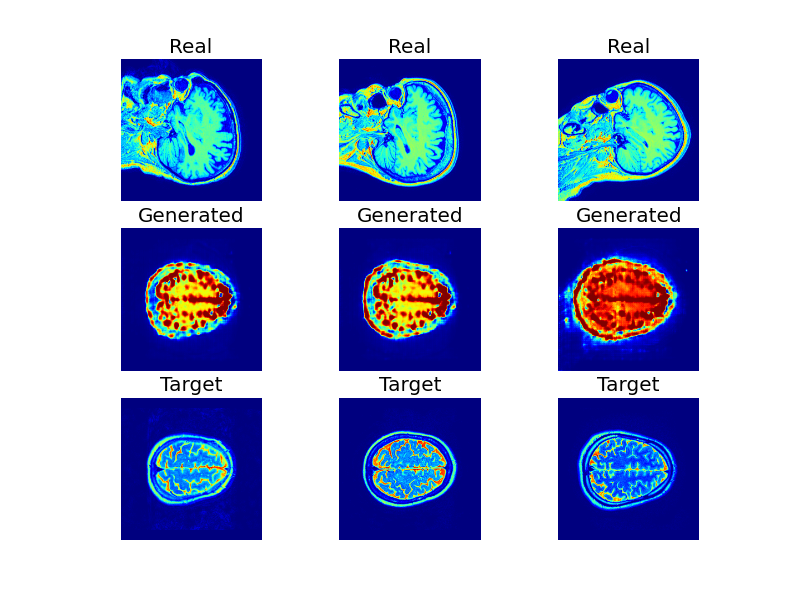
\includegraphics[width=0.95\columnwidth]{plot_004920.png}
    \label{fig:epoch4920}
    \caption{The real, target and generated images after 4920 epoch}
\end{figure}


\begin{figure}[H]
    \centering
    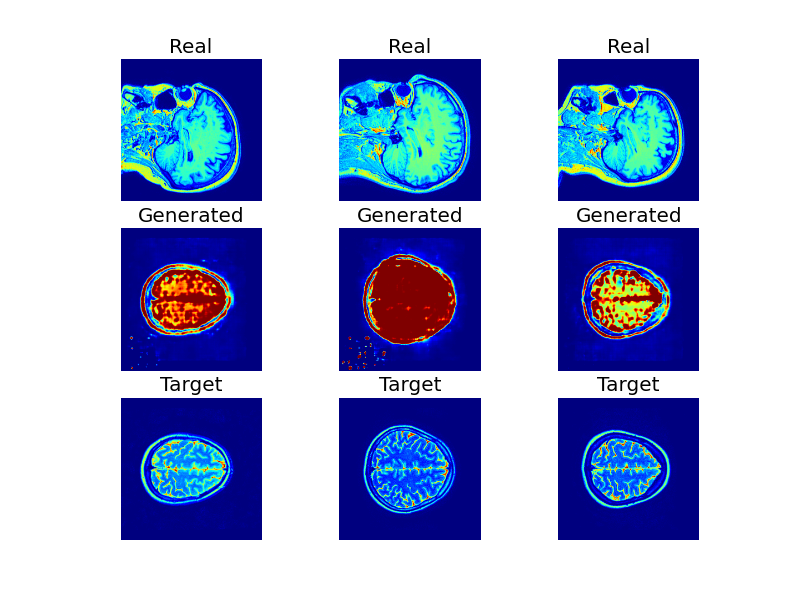
\includegraphics[width=0.95\columnwidth]{plot_029520.png}
    \label{fig:epoch29520}
    \caption{The real, target and generated images after 29520 epochs}
\end{figure}


\begin{figure}[H]
    \centering
    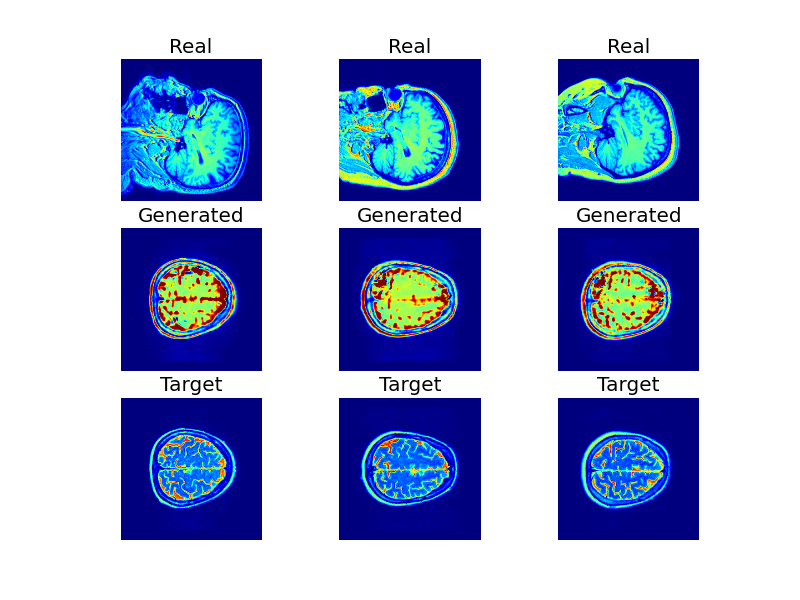
\includegraphics[width=0.95\columnwidth]{plot_049200.png}
    \label{fig:epoch49200}
    \caption{The real, target and generated images after 49200 epoch}
\end{figure}

\section*{Conclusion}

In conclusion, we were able to generate an image from the real and target using the pix2pix GAN. Though the model was able to synthesize the image based on the real and target images, there is still room for improvement. Spending more time on fine-tuning the network, the model should be able to yield far better results which can be indistinguishable from the real images. 

 
\bibliographystyle{IEEEtran}
\bibliography{pix2pix}

\end{document}
